\documentclass[1p]{elsarticle_modified}
%\bibliographystyle{elsarticle-num}

%\usepackage[colorlinks]{hyperref}
%\usepackage{abbrmath_seonhwa} %\Abb, \Ascr, \Acal ,\Abf, \Afrak
\usepackage{amsfonts}
\usepackage{amssymb}
\usepackage{amsmath}
\usepackage{amsthm}
\usepackage{scalefnt}
\usepackage{amsbsy}
\usepackage{kotex}
\usepackage{caption}
\usepackage{subfig}
\usepackage{color}
\usepackage{graphicx}
\usepackage{xcolor} %% white, black, red, green, blue, cyan, magenta, yellow
\usepackage{float}
\usepackage{setspace}
\usepackage{hyperref}

\usepackage{tikz}
\usetikzlibrary{arrows}

\usepackage{multirow}
\usepackage{array} % fixed length table
\usepackage{hhline}

%%%%%%%%%%%%%%%%%%%%%
\makeatletter
\renewcommand*\env@matrix[1][\arraystretch]{%
	\edef\arraystretch{#1}%
	\hskip -\arraycolsep
	\let\@ifnextchar\new@ifnextchar
	\array{*\c@MaxMatrixCols c}}
\makeatother %https://tex.stackexchange.com/questions/14071/how-can-i-increase-the-line-spacing-in-a-matrix
%%%%%%%%%%%%%%%

\usepackage[normalem]{ulem}

\newcommand{\msout}[1]{\ifmmode\text{\sout{\ensuremath{#1}}}\else\sout{#1}\fi}
%SOURCE: \msout is \stkout macro in https://tex.stackexchange.com/questions/20609/strikeout-in-math-mode

\newcommand{\cancel}[1]{
	\ifmmode
	{\color{red}\msout{#1}}
	\else
	{\color{red}\sout{#1}}
	\fi
}

\newcommand{\add}[1]{
	{\color{blue}\uwave{#1}}
}

\newcommand{\replace}[2]{
	\ifmmode
	{\color{red}\msout{#1}}{\color{blue}\uwave{#2}}
	\else
	{\color{red}\sout{#1}}{\color{blue}\uwave{#2}}
	\fi
}

\newcommand{\Sol}{\mathcal{S}} %segment
\newcommand{\D}{D} %diagram
\newcommand{\A}{\mathcal{A}} %arc


%%%%%%%%%%%%%%%%%%%%%%%%%%%%%5 test

\def\sl{\operatorname{\textup{SL}}(2,\Cbb)}
\def\psl{\operatorname{\textup{PSL}}(2,\Cbb)}
\def\quan{\mkern 1mu \triangleright \mkern 1mu}

\theoremstyle{definition}
\newtheorem{thm}{Theorem}[section]
\newtheorem{prop}[thm]{Proposition}
\newtheorem{lem}[thm]{Lemma}
\newtheorem{ques}[thm]{Question}
\newtheorem{cor}[thm]{Corollary}
\newtheorem{defn}[thm]{Definition}
\newtheorem{exam}[thm]{Example}
\newtheorem{rmk}[thm]{Remark}
\newtheorem{alg}[thm]{Algorithm}

\newcommand{\I}{\sqrt{-1}}
\begin{document}

%\begin{frontmatter}
%
%\title{Boundary parabolic representations of knots up to 8 crossings}
%
%%% Group authors per affiliation:
%\author{Yunhi Cho} 
%\address{Department of Mathematics, University of Seoul, Seoul, Korea}
%\ead{yhcho@uos.ac.kr}
%
%
%\author{Seonhwa Kim} %\fnref{s_kim}}
%\address{Center for Geometry and Physics, Institute for Basic Science, Pohang, 37673, Korea}
%\ead{ryeona17@ibs.re.kr}
%
%\author{Hyuk Kim}
%\address{Department of Mathematical Sciences, Seoul National University, Seoul 08826, Korea}
%\ead{hyukkim@snu.ac.kr}
%
%\author{Seokbeom Yoon}
%\address{Department of Mathematical Sciences, Seoul National University, Seoul, 08826,  Korea}
%\ead{sbyoon15@snu.ac.kr}
%
%\begin{abstract}
%We find all boundary parabolic representation of knots up to 8 crossings.
%
%\end{abstract}
%\begin{keyword}
%    \MSC[2010] 57M25 
%\end{keyword}
%
%\end{frontmatter}

%\linenumbers
%\tableofcontents
%
\newcommand\colored[1]{\textcolor{white}{\rule[-0.35ex]{0.8em}{1.4ex}}\kern-0.8em\color{red} #1}%
%\newcommand\colored[1]{\textcolor{white}{ #1}\kern-2.17ex	\textcolor{white}{ #1}\kern-1.81ex	\textcolor{white}{ #1}\kern-2.15ex\color{red}#1	}

{\Large $\underline{12n_{0540}~(K12n_{0540})}$}

\setlength{\tabcolsep}{10pt}
\renewcommand{\arraystretch}{1.6}
\vspace{1cm}\begin{tabular}{m{100pt}>{\centering\arraybackslash}m{274pt}}
\multirow{5}{120pt}{
	\centering
	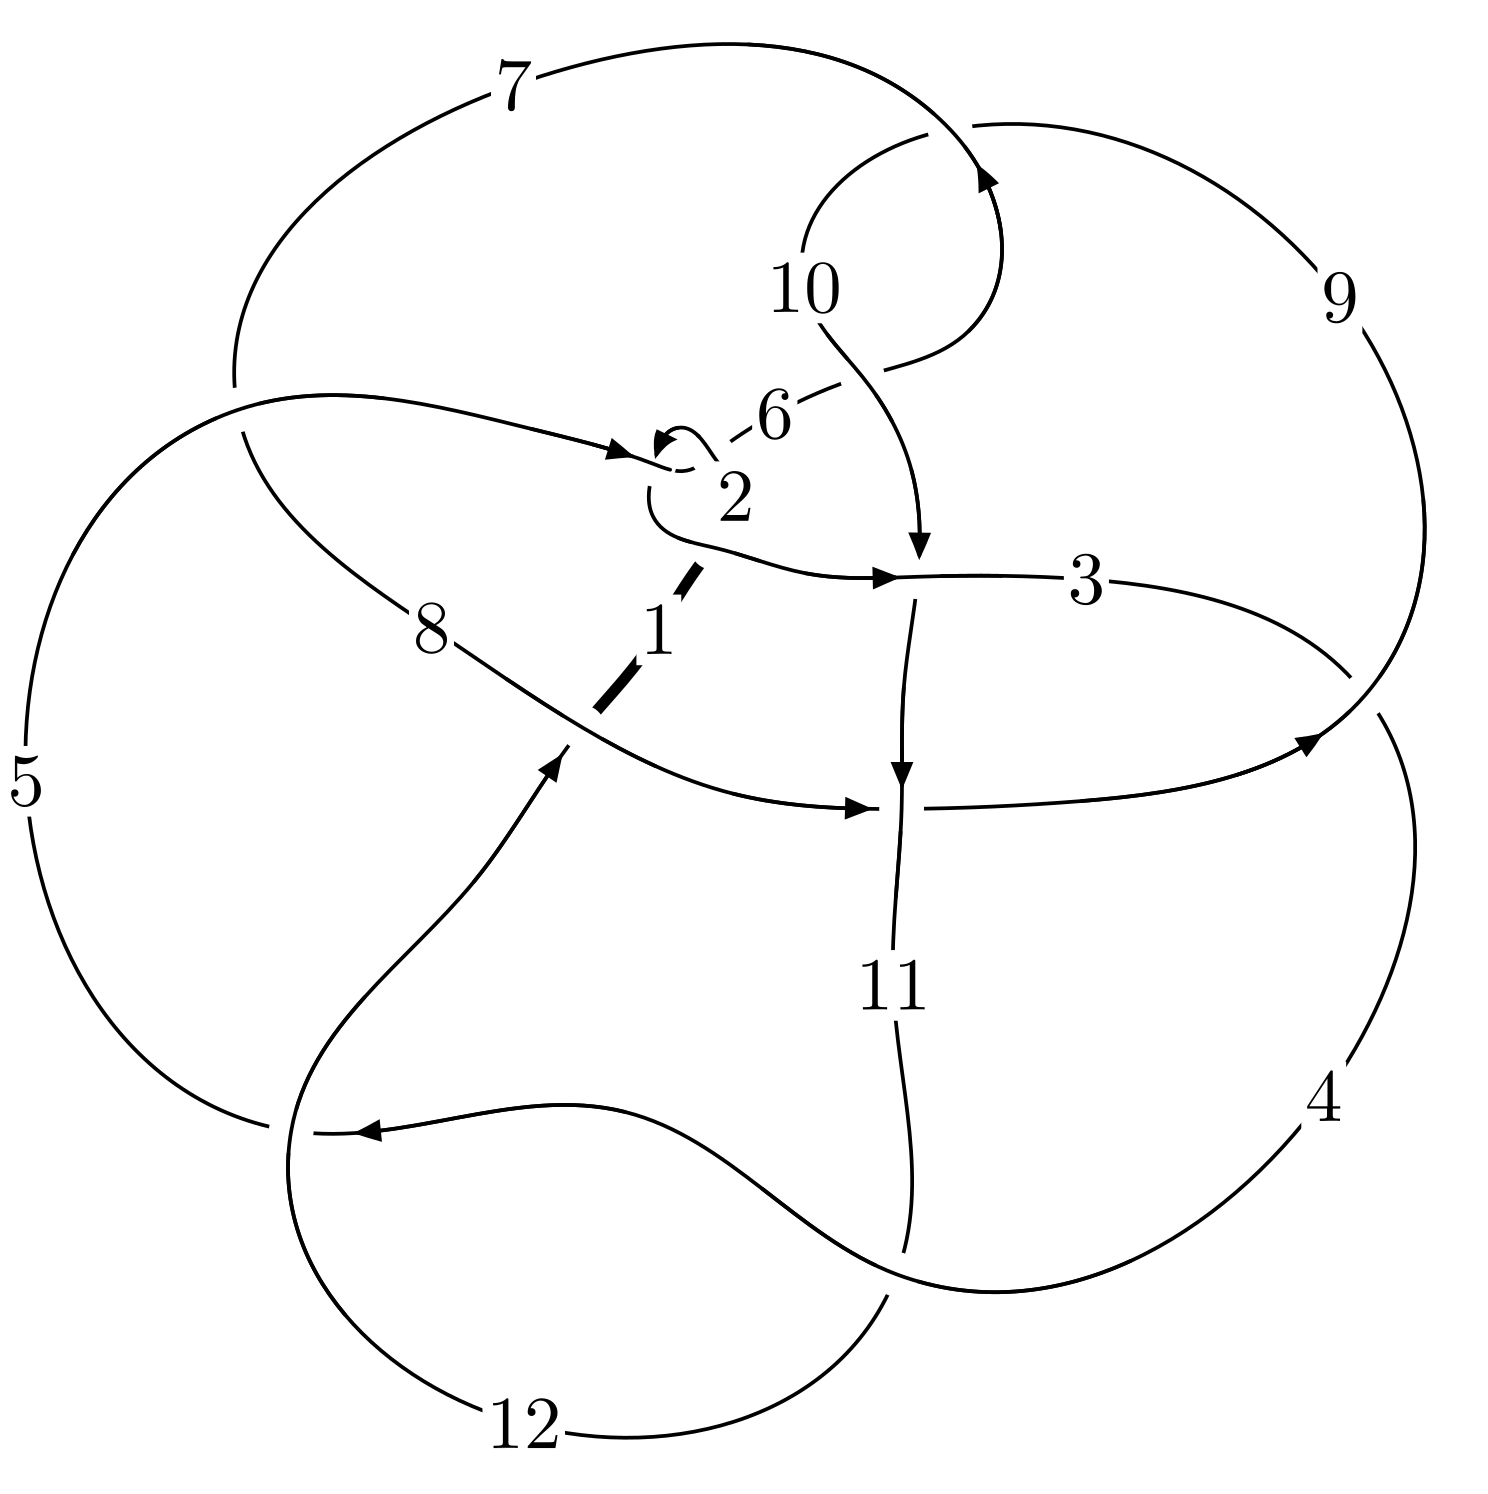
\includegraphics[width=112pt]{../../../GIT/diagram.site/Diagrams/png/2629_12n_0540.png}\\
\ \ \ A knot diagram\footnotemark}&
\allowdisplaybreaks
\textbf{Linearized knot diagam} \\
\cline{2-2}
 &
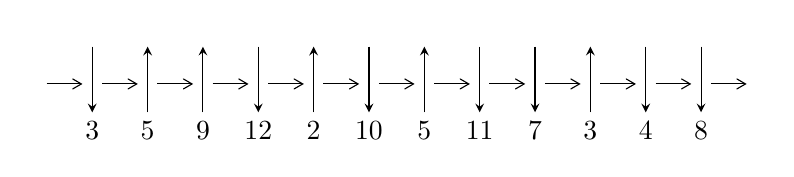
\begin{tikzpicture}[x=20pt, y=17pt]
	% nodes
	\node (C0) at (0, 0) {};
	\node (C1) at (1, 0) {};
	\node (C1U) at (1, +1) {};
	\node (C1D) at (1, -1) {3};

	\node (C2) at (2, 0) {};
	\node (C2U) at (2, +1) {};
	\node (C2D) at (2, -1) {5};

	\node (C3) at (3, 0) {};
	\node (C3U) at (3, +1) {};
	\node (C3D) at (3, -1) {9};

	\node (C4) at (4, 0) {};
	\node (C4U) at (4, +1) {};
	\node (C4D) at (4, -1) {12};

	\node (C5) at (5, 0) {};
	\node (C5U) at (5, +1) {};
	\node (C5D) at (5, -1) {2};

	\node (C6) at (6, 0) {};
	\node (C6U) at (6, +1) {};
	\node (C6D) at (6, -1) {10};

	\node (C7) at (7, 0) {};
	\node (C7U) at (7, +1) {};
	\node (C7D) at (7, -1) {5};

	\node (C8) at (8, 0) {};
	\node (C8U) at (8, +1) {};
	\node (C8D) at (8, -1) {11};

	\node (C9) at (9, 0) {};
	\node (C9U) at (9, +1) {};
	\node (C9D) at (9, -1) {7};

	\node (C10) at (10, 0) {};
	\node (C10U) at (10, +1) {};
	\node (C10D) at (10, -1) {3};

	\node (C11) at (11, 0) {};
	\node (C11U) at (11, +1) {};
	\node (C11D) at (11, -1) {4};

	\node (C12) at (12, 0) {};
	\node (C12U) at (12, +1) {};
	\node (C12D) at (12, -1) {8};
	\node (C13) at (13, 0) {};

	% arrows
	\draw[->,>={angle 60}]
	(C0) edge (C1) (C1) edge (C2) (C2) edge (C3) (C3) edge (C4) (C4) edge (C5) (C5) edge (C6) (C6) edge (C7) (C7) edge (C8) (C8) edge (C9) (C9) edge (C10) (C10) edge (C11) (C11) edge (C12) (C12) edge (C13) ;	\draw[->,>=stealth]
	(C1U) edge (C1D) (C2D) edge (C2U) (C3D) edge (C3U) (C4U) edge (C4D) (C5D) edge (C5U) (C6U) edge (C6D) (C7D) edge (C7U) (C8U) edge (C8D) (C9U) edge (C9D) (C10D) edge (C10U) (C11U) edge (C11D) (C12U) edge (C12D) ;
	\end{tikzpicture} \\
\hhline{~~} \\& 
\textbf{Solving Sequence} \\ \cline{2-2} 
 &
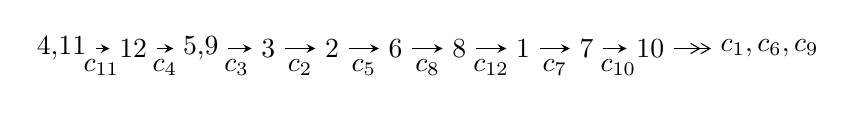
\begin{tikzpicture}[x=23pt, y=7pt]
	% node
	\node (A0) at (-1/8, 0) {4,11};
	\node (A1) at (1, 0) {12};
	\node (A2) at (33/16, 0) {5,9};
	\node (A3) at (25/8, 0) {3};
	\node (A4) at (33/8, 0) {2};
	\node (A5) at (41/8, 0) {6};
	\node (A6) at (49/8, 0) {8};
	\node (A7) at (57/8, 0) {1};
	\node (A8) at (65/8, 0) {7};
	\node (A9) at (73/8, 0) {10};
	\node (C1) at (1/2, -1) {$c_{11}$};
	\node (C2) at (3/2, -1) {$c_{4}$};
	\node (C3) at (21/8, -1) {$c_{3}$};
	\node (C4) at (29/8, -1) {$c_{2}$};
	\node (C5) at (37/8, -1) {$c_{5}$};
	\node (C6) at (45/8, -1) {$c_{8}$};
	\node (C7) at (53/8, -1) {$c_{12}$};
	\node (C8) at (61/8, -1) {$c_{7}$};
	\node (C9) at (69/8, -1) {$c_{10}$};
	\node (A10) at (11, 0) {$c_{1},c_{6},c_{9}$};

	% edge
	\draw[->,>=stealth]	
	(A0) edge (A1) (A1) edge (A2) (A2) edge (A3) (A3) edge (A4) (A4) edge (A5) (A5) edge (A6) (A6) edge (A7) (A7) edge (A8) (A8) edge (A9) ;
	\draw[->>,>={angle 60}]	
	(A9) edge (A10);
\end{tikzpicture} \\ 

\end{tabular} \\

\footnotetext{
The image of knot diagram is generated by the software ``\textbf{Draw programme}" developed by Andrew Bartholomew(\url{http://www.layer8.co.uk/maths/draw/index.htm\#Running-draw}), where we modified some parts for our purpose(\url{https://github.com/CATsTAILs/LinksPainter}).
}\phantom \\ \newline 
\centering \textbf{Ideals for irreducible components\footnotemark of $X_{\text{par}}$} 
 
\begin{align*}
I^u_{1}&=\langle 
-3.47946\times10^{114} u^{67}+5.80911\times10^{114} u^{66}+\cdots+2.34165\times10^{114} b+9.83922\times10^{115},\\
\phantom{I^u_{1}}&\phantom{= \langle  }1.83497\times10^{116} u^{67}-3.18289\times10^{116} u^{66}+\cdots+1.63915\times10^{115} a-6.53773\times10^{117},\\
\phantom{I^u_{1}}&\phantom{= \langle  }u^{68}-2 u^{67}+\cdots-116 u+7\rangle \\
I^u_{2}&=\langle 
5848837527 u^{22}+13674615497 u^{21}+\cdots+52233066871 b+111138789648,\\
\phantom{I^u_{2}}&\phantom{= \langle  }7655480010 u^{22}+231901700034 u^{21}+\cdots+679029869323 a+1495389378052,\\
\phantom{I^u_{2}}&\phantom{= \langle  }u^{23}- u^{22}+\cdots+7 u-13\rangle \\
\\
\end{align*}
\raggedright * 2 irreducible components of $\dim_{\mathbb{C}}=0$, with total 91 representations.\\
\footnotetext{All coefficients of polynomials are rational numbers. But the coefficients are sometimes approximated in decimal forms when there is not enough margin.}
\newpage
\renewcommand{\arraystretch}{1}
\centering \section*{I. $I^u_{1}= \langle -3.48\times10^{114} u^{67}+5.81\times10^{114} u^{66}+\cdots+2.34\times10^{114} b+9.84\times10^{115},\;1.83\times10^{116} u^{67}-3.18\times10^{116} u^{66}+\cdots+1.64\times10^{115} a-6.54\times10^{117},\;u^{68}-2 u^{67}+\cdots-116 u+7 \rangle$}
\flushleft \textbf{(i) Arc colorings}\\
\begin{tabular}{m{7pt} m{180pt} m{7pt} m{180pt} }
\flushright $a_{4}=$&$\begin{pmatrix}0\\u\end{pmatrix}$ \\
\flushright $a_{11}=$&$\begin{pmatrix}1\\0\end{pmatrix}$ \\
\flushright $a_{12}=$&$\begin{pmatrix}1\\u^2\end{pmatrix}$ \\
\flushright $a_{5}=$&$\begin{pmatrix}- u\\- u^3+u\end{pmatrix}$ \\
\flushright $a_{9}=$&$\begin{pmatrix}-11.1946 u^{67}+19.4179 u^{66}+\cdots-4458.06 u+398.848\\1.48590 u^{67}-2.48078 u^{66}+\cdots+478.228 u-42.0184\end{pmatrix}$ \\
\flushright $a_{3}=$&$\begin{pmatrix}2.99528 u^{67}-8.06816 u^{66}+\cdots+2059.11 u-186.296\\-2.40290 u^{67}+3.48812 u^{66}+\cdots-722.342 u+62.8761\end{pmatrix}$ \\
\flushright $a_{2}=$&$\begin{pmatrix}2.86290 u^{67}-7.77263 u^{66}+\cdots+1979.48 u-179.800\\-1.95630 u^{67}+3.03856 u^{66}+\cdots-638.210 u+56.1653\end{pmatrix}$ \\
\flushright $a_{6}=$&$\begin{pmatrix}6.23282 u^{67}-9.22792 u^{66}+\cdots+1916.42 u-165.385\\0.664956 u^{67}-0.0247150 u^{66}+\cdots-88.8156 u+11.7141\end{pmatrix}$ \\
\flushright $a_{8}=$&$\begin{pmatrix}-9.70871 u^{67}+16.9371 u^{66}+\cdots-3979.83 u+356.830\\1.48590 u^{67}-2.48078 u^{66}+\cdots+478.228 u-42.0184\end{pmatrix}$ \\
\flushright $a_{1}=$&$\begin{pmatrix}3.04846 u^{67}-9.72123 u^{66}+\cdots+2742.54 u-254.243\\-2.53855 u^{67}+3.80062 u^{66}+\cdots-783.316 u+67.5088\end{pmatrix}$ \\
\flushright $a_{7}=$&$\begin{pmatrix}-10.5542 u^{67}+17.7616 u^{66}+\cdots-3993.89 u+354.809\\1.59941 u^{67}-2.25196 u^{66}+\cdots+397.680 u-33.9317\end{pmatrix}$ \\
\flushright $a_{10}=$&$\begin{pmatrix}-2.77331 u^{67}+5.28127 u^{66}+\cdots-1350.34 u+125.631\\1.09656 u^{67}-0.524123 u^{66}+\cdots-2.65244 u+2.93062\end{pmatrix}$\\&\end{tabular}
\flushleft \textbf{(ii) Obstruction class $= -1$}\\~\\
\flushleft \textbf{(iii) Cusp Shapes $= -3.24479 u^{67}+8.28537 u^{66}+\cdots-1873.76 u+165.568$}\\~\\
\newpage\renewcommand{\arraystretch}{1}
\flushleft \textbf{(iv) u-Polynomials at the component}\newline \\
\begin{tabular}{m{50pt}|m{274pt}}
Crossings & \hspace{64pt}u-Polynomials at each crossing \\
\hline $$\begin{aligned}c_{1}\end{aligned}$$&$\begin{aligned}
&u^{68}+83 u^{67}+\cdots+50717133 u+1247689
\end{aligned}$\\
\hline $$\begin{aligned}c_{2},c_{5}\end{aligned}$$&$\begin{aligned}
&u^{68}+3 u^{67}+\cdots+2197 u+1117
\end{aligned}$\\
\hline $$\begin{aligned}c_{3}\end{aligned}$$&$\begin{aligned}
&u^{68}+u^{67}+\cdots+3064 u+911
\end{aligned}$\\
\hline $$\begin{aligned}c_{4},c_{11}\end{aligned}$$&$\begin{aligned}
&u^{68}+2 u^{67}+\cdots+116 u+7
\end{aligned}$\\
\hline $$\begin{aligned}c_{6},c_{9}\end{aligned}$$&$\begin{aligned}
&u^{68}+4 u^{67}+\cdots-34 u+3
\end{aligned}$\\
\hline $$\begin{aligned}c_{7}\end{aligned}$$&$\begin{aligned}
&u^{68}+12 u^{67}+\cdots+789947 u+129293
\end{aligned}$\\
\hline $$\begin{aligned}c_{8}\end{aligned}$$&$\begin{aligned}
&u^{68}-9 u^{66}+\cdots-28 u+88
\end{aligned}$\\
\hline $$\begin{aligned}c_{10}\end{aligned}$$&$\begin{aligned}
&u^{68}-2 u^{67}+\cdots+1328829 u+2269219
\end{aligned}$\\
\hline $$\begin{aligned}c_{12}\end{aligned}$$&$\begin{aligned}
&u^{68}+u^{67}+\cdots-3738678 u+370609
\end{aligned}$\\
\hline
\end{tabular}\\~\\
\newpage\renewcommand{\arraystretch}{1}
\flushleft \textbf{(v) Riley Polynomials at the component}\newline \\
\begin{tabular}{m{50pt}|m{274pt}}
Crossings & \hspace{64pt}Riley Polynomials at each crossing \\
\hline $$\begin{aligned}c_{1}\end{aligned}$$&$\begin{aligned}
&y^{68}-177 y^{67}+\cdots-202908028705639 y+1556727840721
\end{aligned}$\\
\hline $$\begin{aligned}c_{2},c_{5}\end{aligned}$$&$\begin{aligned}
&y^{68}+83 y^{67}+\cdots+50717133 y+1247689
\end{aligned}$\\
\hline $$\begin{aligned}c_{3}\end{aligned}$$&$\begin{aligned}
&y^{68}+21 y^{67}+\cdots+24920164 y+829921
\end{aligned}$\\
\hline $$\begin{aligned}c_{4},c_{11}\end{aligned}$$&$\begin{aligned}
&y^{68}-48 y^{67}+\cdots-2858 y+49
\end{aligned}$\\
\hline $$\begin{aligned}c_{6},c_{9}\end{aligned}$$&$\begin{aligned}
&y^{68}+8 y^{67}+\cdots-220 y+9
\end{aligned}$\\
\hline $$\begin{aligned}c_{7}\end{aligned}$$&$\begin{aligned}
&y^{68}+68 y^{67}+\cdots+2855259918707 y+16716679849
\end{aligned}$\\
\hline $$\begin{aligned}c_{8}\end{aligned}$$&$\begin{aligned}
&y^{68}-18 y^{67}+\cdots+160432 y+7744
\end{aligned}$\\
\hline $$\begin{aligned}c_{10}\end{aligned}$$&$\begin{aligned}
&y^{68}+52 y^{67}+\cdots+220850551819415 y+5149354869961
\end{aligned}$\\
\hline $$\begin{aligned}c_{12}\end{aligned}$$&$\begin{aligned}
&y^{68}-45 y^{67}+\cdots-1916711732460 y+137351030881
\end{aligned}$\\
\hline
\end{tabular}\\~\\
\newpage\flushleft \textbf{(vi) Complex Volumes and Cusp Shapes}
$$\begin{array}{c|c|c}  
\text{Solutions to }I^u_{1}& \I (\text{vol} + \sqrt{-1}CS) & \text{Cusp shape}\\
 \hline 
\begin{aligned}
u &= \phantom{-}0.947765 + 0.357665 I \\
a &= \phantom{-}0.040563 + 1.213920 I \\
b &= -0.628775 - 0.554793 I\end{aligned}
 & -1.10242 - 1.88768 I & \phantom{-0.000000 } 0 \\ \hline\begin{aligned}
u &= \phantom{-}0.947765 - 0.357665 I \\
a &= \phantom{-}0.040563 - 1.213920 I \\
b &= -0.628775 + 0.554793 I\end{aligned}
 & -1.10242 + 1.88768 I & \phantom{-0.000000 } 0 \\ \hline\begin{aligned}
u &= -0.206261 + 1.007020 I \\
a &= \phantom{-}0.906803 - 0.883651 I \\
b &= -1.166080 + 0.709081 I\end{aligned}
 & -9.04368 + 2.56194 I & \phantom{-0.000000 } 0 \\ \hline\begin{aligned}
u &= -0.206261 - 1.007020 I \\
a &= \phantom{-}0.906803 + 0.883651 I \\
b &= -1.166080 - 0.709081 I\end{aligned}
 & -9.04368 - 2.56194 I & \phantom{-0.000000 } 0 \\ \hline\begin{aligned}
u &= -0.952275 + 0.015155 I \\
a &= -0.389347 + 1.110760 I \\
b &= -1.51867 - 0.44627 I\end{aligned}
 & -6.56999 + 0.14060 I & -5.76756 + 0. I\phantom{ +0.000000I} \\ \hline\begin{aligned}
u &= -0.952275 - 0.015155 I \\
a &= -0.389347 - 1.110760 I \\
b &= -1.51867 + 0.44627 I\end{aligned}
 & -6.56999 - 0.14060 I & -5.76756 + 0. I\phantom{ +0.000000I} \\ \hline\begin{aligned}
u &= \phantom{-}0.119156 + 1.120550 I \\
a &= \phantom{-}0.632936 + 0.272438 I \\
b &= -0.526423 + 0.033002 I\end{aligned}
 & \phantom{-}0.601823 - 0.891457 I & \phantom{-0.000000 } 0 \\ \hline\begin{aligned}
u &= \phantom{-}0.119156 - 1.120550 I \\
a &= \phantom{-}0.632936 - 0.272438 I \\
b &= -0.526423 - 0.033002 I\end{aligned}
 & \phantom{-}0.601823 + 0.891457 I & \phantom{-0.000000 } 0 \\ \hline\begin{aligned}
u &= \phantom{-}1.131540 + 0.066351 I \\
a &= -1.34290 - 1.03710 I \\
b &= -0.842012 + 0.236969 I\end{aligned}
 & -3.61434 - 1.69153 I & \phantom{-0.000000 } 0 \\ \hline\begin{aligned}
u &= \phantom{-}1.131540 - 0.066351 I \\
a &= -1.34290 + 1.03710 I \\
b &= -0.842012 - 0.236969 I\end{aligned}
 & -3.61434 + 1.69153 I & \phantom{-0.000000 } 0\\
 \hline 
 \end{array}$$\newpage$$\begin{array}{c|c|c}  
\text{Solutions to }I^u_{1}& \I (\text{vol} + \sqrt{-1}CS) & \text{Cusp shape}\\
 \hline 
\begin{aligned}
u &= \phantom{-}1.125430 + 0.171124 I \\
a &= -0.153836 + 0.563315 I \\
b &= \phantom{-}1.11877 - 2.59647 I\end{aligned}
 & -10.13300 - 5.69758 I & \phantom{-0.000000 } 0 \\ \hline\begin{aligned}
u &= \phantom{-}1.125430 - 0.171124 I \\
a &= -0.153836 - 0.563315 I \\
b &= \phantom{-}1.11877 + 2.59647 I\end{aligned}
 & -10.13300 + 5.69758 I & \phantom{-0.000000 } 0 \\ \hline\begin{aligned}
u &= \phantom{-}0.175099 + 0.838478 I \\
a &= \phantom{-}0.638073 + 0.706860 I \\
b &= -0.333831 - 0.671397 I\end{aligned}
 & \phantom{-}0.31102 - 1.89447 I & -2.64082 + 6.58964 I \\ \hline\begin{aligned}
u &= \phantom{-}0.175099 - 0.838478 I \\
a &= \phantom{-}0.638073 - 0.706860 I \\
b &= -0.333831 + 0.671397 I\end{aligned}
 & \phantom{-}0.31102 + 1.89447 I & -2.64082 - 6.58964 I \\ \hline\begin{aligned}
u &= -1.088590 + 0.350394 I \\
a &= \phantom{-}0.578583 + 0.954503 I \\
b &= \phantom{-}1.31358 - 0.94934 I\end{aligned}
 & \phantom{-}1.42621 + 5.22038 I & \phantom{-0.000000 } 0 \\ \hline\begin{aligned}
u &= -1.088590 - 0.350394 I \\
a &= \phantom{-}0.578583 - 0.954503 I \\
b &= \phantom{-}1.31358 + 0.94934 I\end{aligned}
 & \phantom{-}1.42621 - 5.22038 I & \phantom{-0.000000 } 0 \\ \hline\begin{aligned}
u &= \phantom{-}1.141830 + 0.179993 I \\
a &= \phantom{-}0.82568 - 1.37936 I \\
b &= \phantom{-}0.908474 + 0.921235 I\end{aligned}
 & -0.61521 - 4.20240 I & \phantom{-0.000000 } 0 \\ \hline\begin{aligned}
u &= \phantom{-}1.141830 - 0.179993 I \\
a &= \phantom{-}0.82568 + 1.37936 I \\
b &= \phantom{-}0.908474 - 0.921235 I\end{aligned}
 & -0.61521 + 4.20240 I & \phantom{-0.000000 } 0 \\ \hline\begin{aligned}
u &= -0.043094 + 1.162240 I \\
a &= -0.911498 + 0.621527 I \\
b &= \phantom{-}1.098450 - 0.740956 I\end{aligned}
 & -8.72944 + 10.14780 I & \phantom{-0.000000 } 0 \\ \hline\begin{aligned}
u &= -0.043094 - 1.162240 I \\
a &= -0.911498 - 0.621527 I \\
b &= \phantom{-}1.098450 + 0.740956 I\end{aligned}
 & -8.72944 - 10.14780 I & \phantom{-0.000000 } 0\\
 \hline 
 \end{array}$$\newpage$$\begin{array}{c|c|c}  
\text{Solutions to }I^u_{1}& \I (\text{vol} + \sqrt{-1}CS) & \text{Cusp shape}\\
 \hline 
\begin{aligned}
u &= \phantom{-}0.730243 + 0.911092 I \\
a &= \phantom{-}0.436558 - 0.057088 I \\
b &= -0.035935 + 0.195728 I\end{aligned}
 & -0.33349 - 2.89073 I & \phantom{-0.000000 } 0 \\ \hline\begin{aligned}
u &= \phantom{-}0.730243 - 0.911092 I \\
a &= \phantom{-}0.436558 + 0.057088 I \\
b &= -0.035935 - 0.195728 I\end{aligned}
 & -0.33349 + 2.89073 I & \phantom{-0.000000 } 0 \\ \hline\begin{aligned}
u &= -1.180250 + 0.039699 I \\
a &= -0.322263 - 0.642592 I \\
b &= -1.36957 + 0.98710 I\end{aligned}
 & -4.90609 + 1.45309 I & \phantom{-0.000000 } 0 \\ \hline\begin{aligned}
u &= -1.180250 - 0.039699 I \\
a &= -0.322263 + 0.642592 I \\
b &= -1.36957 - 0.98710 I\end{aligned}
 & -4.90609 - 1.45309 I & \phantom{-0.000000 } 0 \\ \hline\begin{aligned}
u &= -1.176600 + 0.191135 I \\
a &= -1.93965 + 0.51920 I \\
b &= -0.695306 + 0.367890 I\end{aligned}
 & -10.52210 + 6.41640 I & \phantom{-0.000000 } 0 \\ \hline\begin{aligned}
u &= -1.176600 - 0.191135 I \\
a &= -1.93965 - 0.51920 I \\
b &= -0.695306 - 0.367890 I\end{aligned}
 & -10.52210 - 6.41640 I & \phantom{-0.000000 } 0 \\ \hline\begin{aligned}
u &= \phantom{-}0.060621 + 1.190540 I \\
a &= -0.571573 - 0.371721 I \\
b &= \phantom{-}0.867630 + 0.303277 I\end{aligned}
 & -0.46876 - 4.20757 I & \phantom{-0.000000 } 0 \\ \hline\begin{aligned}
u &= \phantom{-}0.060621 - 1.190540 I \\
a &= -0.571573 + 0.371721 I \\
b &= \phantom{-}0.867630 - 0.303277 I\end{aligned}
 & -0.46876 + 4.20757 I & \phantom{-0.000000 } 0 \\ \hline\begin{aligned}
u &= -1.182210 + 0.170919 I \\
a &= \phantom{-}0.088084 - 0.589191 I \\
b &= \phantom{-}0.714259 + 1.051810 I\end{aligned}
 & -2.89595 + 4.08070 I & \phantom{-0.000000 } 0 \\ \hline\begin{aligned}
u &= -1.182210 - 0.170919 I \\
a &= \phantom{-}0.088084 + 0.589191 I \\
b &= \phantom{-}0.714259 - 1.051810 I\end{aligned}
 & -2.89595 - 4.08070 I & \phantom{-0.000000 } 0\\
 \hline 
 \end{array}$$\newpage$$\begin{array}{c|c|c}  
\text{Solutions to }I^u_{1}& \I (\text{vol} + \sqrt{-1}CS) & \text{Cusp shape}\\
 \hline 
\begin{aligned}
u &= -0.404834 + 0.685829 I \\
a &= -0.940474 - 0.323677 I \\
b &= \phantom{-}0.693348 + 0.865586 I\end{aligned}
 & \phantom{-}3.55477 - 1.28710 I & \phantom{-}5.05160 + 1.04556 I \\ \hline\begin{aligned}
u &= -0.404834 - 0.685829 I \\
a &= -0.940474 + 0.323677 I \\
b &= \phantom{-}0.693348 - 0.865586 I\end{aligned}
 & \phantom{-}3.55477 + 1.28710 I & \phantom{-}5.05160 - 1.04556 I \\ \hline\begin{aligned}
u &= \phantom{-}1.223450 + 0.114208 I \\
a &= \phantom{-}0.838650 + 0.592410 I \\
b &= \phantom{-}0.466055 - 0.033333 I\end{aligned}
 & -3.07031 - 0.92088 I & \phantom{-0.000000 } 0 \\ \hline\begin{aligned}
u &= \phantom{-}1.223450 - 0.114208 I \\
a &= \phantom{-}0.838650 - 0.592410 I \\
b &= \phantom{-}0.466055 + 0.033333 I\end{aligned}
 & -3.07031 + 0.92088 I & \phantom{-0.000000 } 0 \\ \hline\begin{aligned}
u &= \phantom{-}1.242620 + 0.025631 I \\
a &= \phantom{-}0.032890 - 0.504754 I \\
b &= -1.72206 + 2.06580 I\end{aligned}
 & -11.42940 + 2.92629 I & \phantom{-0.000000 } 0 \\ \hline\begin{aligned}
u &= \phantom{-}1.242620 - 0.025631 I \\
a &= \phantom{-}0.032890 + 0.504754 I \\
b &= -1.72206 - 2.06580 I\end{aligned}
 & -11.42940 - 2.92629 I & \phantom{-0.000000 } 0 \\ \hline\begin{aligned}
u &= -1.275810 + 0.008672 I \\
a &= \phantom{-}1.30907 + 1.34723 I \\
b &= \phantom{-}0.772778 + 0.039008 I\end{aligned}
 & -12.42140 + 2.86949 I & \phantom{-0.000000 } 0 \\ \hline\begin{aligned}
u &= -1.275810 - 0.008672 I \\
a &= \phantom{-}1.30907 - 1.34723 I \\
b &= \phantom{-}0.772778 - 0.039008 I\end{aligned}
 & -12.42140 - 2.86949 I & \phantom{-0.000000 } 0 \\ \hline\begin{aligned}
u &= \phantom{-}1.091170 + 0.758270 I \\
a &= -0.048055 - 0.621973 I \\
b &= \phantom{-}1.388680 + 0.122425 I\end{aligned}
 & -5.10581 - 3.43321 I & \phantom{-0.000000 } 0 \\ \hline\begin{aligned}
u &= \phantom{-}1.091170 - 0.758270 I \\
a &= -0.048055 + 0.621973 I \\
b &= \phantom{-}1.388680 - 0.122425 I\end{aligned}
 & -5.10581 + 3.43321 I & \phantom{-0.000000 } 0\\
 \hline 
 \end{array}$$\newpage$$\begin{array}{c|c|c}  
\text{Solutions to }I^u_{1}& \I (\text{vol} + \sqrt{-1}CS) & \text{Cusp shape}\\
 \hline 
\begin{aligned}
u &= -1.269780 + 0.488456 I \\
a &= \phantom{-}0.006811 - 1.078700 I \\
b &= -0.742033 + 0.701033 I\end{aligned}
 & -3.69503 + 6.20269 I & \phantom{-0.000000 } 0 \\ \hline\begin{aligned}
u &= -1.269780 - 0.488456 I \\
a &= \phantom{-}0.006811 + 1.078700 I \\
b &= -0.742033 - 0.701033 I\end{aligned}
 & -3.69503 - 6.20269 I & \phantom{-0.000000 } 0 \\ \hline\begin{aligned}
u &= \phantom{-}0.011349 + 0.622403 I \\
a &= \phantom{-}0.565810 + 1.046550 I \\
b &= \phantom{-}0.180164 - 0.381969 I\end{aligned}
 & \phantom{-}0.84600 - 1.53956 I & \phantom{-}1.33813 + 2.18949 I \\ \hline\begin{aligned}
u &= \phantom{-}0.011349 - 0.622403 I \\
a &= \phantom{-}0.565810 - 1.046550 I \\
b &= \phantom{-}0.180164 + 0.381969 I\end{aligned}
 & \phantom{-}0.84600 + 1.53956 I & \phantom{-}1.33813 - 2.18949 I \\ \hline\begin{aligned}
u &= \phantom{-}1.38641 + 0.42602 I \\
a &= -0.380161 + 1.136250 I \\
b &= -1.45552 - 0.92583 I\end{aligned}
 & -14.0339 - 7.5741 I & \phantom{-0.000000 } 0 \\ \hline\begin{aligned}
u &= \phantom{-}1.38641 - 0.42602 I \\
a &= -0.380161 - 1.136250 I \\
b &= -1.45552 + 0.92583 I\end{aligned}
 & -14.0339 + 7.5741 I & \phantom{-0.000000 } 0 \\ \hline\begin{aligned}
u &= -1.38018 + 0.44717 I \\
a &= -0.180863 - 0.851166 I \\
b &= -1.05821 + 1.05211 I\end{aligned}
 & -4.53688 + 6.71623 I & \phantom{-0.000000 } 0 \\ \hline\begin{aligned}
u &= -1.38018 - 0.44717 I \\
a &= -0.180863 + 0.851166 I \\
b &= -1.05821 - 1.05211 I\end{aligned}
 & -4.53688 - 6.71623 I & \phantom{-0.000000 } 0 \\ \hline\begin{aligned}
u &= -1.30930 + 0.68061 I \\
a &= \phantom{-}0.466558 - 0.599062 I \\
b &= -1.119230 - 0.290691 I\end{aligned}
 & -12.20000 + 3.56524 I & \phantom{-0.000000 } 0 \\ \hline\begin{aligned}
u &= -1.30930 - 0.68061 I \\
a &= \phantom{-}0.466558 + 0.599062 I \\
b &= -1.119230 + 0.290691 I\end{aligned}
 & -12.20000 - 3.56524 I & \phantom{-0.000000 } 0\\
 \hline 
 \end{array}$$\newpage$$\begin{array}{c|c|c}  
\text{Solutions to }I^u_{1}& \I (\text{vol} + \sqrt{-1}CS) & \text{Cusp shape}\\
 \hline 
\begin{aligned}
u &= -1.39983 + 0.51827 I \\
a &= \phantom{-}0.251477 + 0.976417 I \\
b &= \phantom{-}1.203380 - 0.632990 I\end{aligned}
 & -5.13007 + 10.12020 I & \phantom{-0.000000 } 0 \\ \hline\begin{aligned}
u &= -1.39983 - 0.51827 I \\
a &= \phantom{-}0.251477 - 0.976417 I \\
b &= \phantom{-}1.203380 + 0.632990 I\end{aligned}
 & -5.13007 - 10.12020 I & \phantom{-0.000000 } 0 \\ \hline\begin{aligned}
u &= \phantom{-}1.39753 + 0.53362 I \\
a &= \phantom{-}0.246829 - 1.107490 I \\
b &= \phantom{-}1.48762 + 0.95191 I\end{aligned}
 & -13.2811 - 16.0932 I & \phantom{-0.000000 } 0 \\ \hline\begin{aligned}
u &= \phantom{-}1.39753 - 0.53362 I \\
a &= \phantom{-}0.246829 + 1.107490 I \\
b &= \phantom{-}1.48762 - 0.95191 I\end{aligned}
 & -13.2811 + 16.0932 I & \phantom{-0.000000 } 0 \\ \hline\begin{aligned}
u &= \phantom{-}1.40478 + 0.55900 I \\
a &= \phantom{-}0.067000 + 0.648345 I \\
b &= -1.010050 - 0.582448 I\end{aligned}
 & -3.60803 - 5.31106 I & \phantom{-0.000000 } 0 \\ \hline\begin{aligned}
u &= \phantom{-}1.40478 - 0.55900 I \\
a &= \phantom{-}0.067000 - 0.648345 I \\
b &= -1.010050 + 0.582448 I\end{aligned}
 & -3.60803 + 5.31106 I & \phantom{-0.000000 } 0 \\ \hline\begin{aligned}
u &= \phantom{-}1.44778 + 0.50507 I \\
a &= \phantom{-}0.107561 - 0.627005 I \\
b &= \phantom{-}1.060660 + 0.226591 I\end{aligned}
 & -5.13201 - 2.07157 I & \phantom{-0.000000 } 0 \\ \hline\begin{aligned}
u &= \phantom{-}1.44778 - 0.50507 I \\
a &= \phantom{-}0.107561 + 0.627005 I \\
b &= \phantom{-}1.060660 - 0.226591 I\end{aligned}
 & -5.13201 + 2.07157 I & \phantom{-0.000000 } 0 \\ \hline\begin{aligned}
u &= \phantom{-}0.373319 + 0.206165 I \\
a &= -2.73778 - 0.45710 I \\
b &= \phantom{-}0.508605 - 0.537274 I\end{aligned}
 & \phantom{-}1.78723 + 2.33202 I & -4.39316 - 1.89690 I \\ \hline\begin{aligned}
u &= \phantom{-}0.373319 - 0.206165 I \\
a &= -2.73778 + 0.45710 I \\
b &= \phantom{-}0.508605 + 0.537274 I\end{aligned}
 & \phantom{-}1.78723 - 2.33202 I & -4.39316 + 1.89690 I\\
 \hline 
 \end{array}$$\newpage$$\begin{array}{c|c|c}  
\text{Solutions to }I^u_{1}& \I (\text{vol} + \sqrt{-1}CS) & \text{Cusp shape}\\
 \hline 
\begin{aligned}
u &= \phantom{-}0.249284 + 0.339745 I \\
a &= \phantom{-}2.71001 - 0.73800 I \\
b &= \phantom{-}0.947188 + 1.031140 I\end{aligned}
 & -7.68973 + 3.58621 I & -2.25293 - 1.72671 I \\ \hline\begin{aligned}
u &= \phantom{-}0.249284 - 0.339745 I \\
a &= \phantom{-}2.71001 + 0.73800 I \\
b &= \phantom{-}0.947188 - 1.031140 I\end{aligned}
 & -7.68973 - 3.58621 I & -2.25293 + 1.72671 I \\ \hline\begin{aligned}
u &= -1.47747 + 0.55770 I \\
a &= -0.303874 + 0.589982 I \\
b &= \phantom{-}0.961351 + 0.168628 I\end{aligned}
 & -13.22700 - 3.78980 I & \phantom{-0.000000 } 0 \\ \hline\begin{aligned}
u &= -1.47747 - 0.55770 I \\
a &= -0.303874 - 0.589982 I \\
b &= \phantom{-}0.961351 - 0.168628 I\end{aligned}
 & -13.22700 + 3.78980 I & \phantom{-0.000000 } 0 \\ \hline\begin{aligned}
u &= -0.097604 + 0.392483 I \\
a &= -1.27273 + 2.72091 I \\
b &= -0.788066 - 1.085820 I\end{aligned}
 & -7.38084 - 4.11631 I & -1.81227 + 1.53073 I \\ \hline\begin{aligned}
u &= -0.097604 - 0.392483 I \\
a &= -1.27273 - 2.72091 I \\
b &= -0.788066 + 1.085820 I\end{aligned}
 & -7.38084 + 4.11631 I & -1.81227 - 1.53073 I \\ \hline\begin{aligned}
u &= \phantom{-}0.184696 + 0.005265 I \\
a &= \phantom{-}1.31649 - 3.97124 I \\
b &= -0.679221 + 0.376391 I\end{aligned}
 & -1.19167 + 1.07394 I & -6.06832 - 1.82745 I \\ \hline\begin{aligned}
u &= \phantom{-}0.184696 - 0.005265 I \\
a &= \phantom{-}1.31649 + 3.97124 I \\
b &= -0.679221 - 0.376391 I\end{aligned}
 & -1.19167 - 1.07394 I & -6.06832 + 1.82745 I\\
 \hline 
 \end{array}$$\newpage\newpage\renewcommand{\arraystretch}{1}
\centering \section*{II. $I^u_{2}= \langle 5.85\times10^{9} u^{22}+1.37\times10^{10} u^{21}+\cdots+5.22\times10^{10} b+1.11\times10^{11},\;7.66\times10^{9} u^{22}+2.32\times10^{11} u^{21}+\cdots+6.79\times10^{11} a+1.50\times10^{12},\;u^{23}- u^{22}+\cdots+7 u-13 \rangle$}
\flushleft \textbf{(i) Arc colorings}\\
\begin{tabular}{m{7pt} m{180pt} m{7pt} m{180pt} }
\flushright $a_{4}=$&$\begin{pmatrix}0\\u\end{pmatrix}$ \\
\flushright $a_{11}=$&$\begin{pmatrix}1\\0\end{pmatrix}$ \\
\flushright $a_{12}=$&$\begin{pmatrix}1\\u^2\end{pmatrix}$ \\
\flushright $a_{5}=$&$\begin{pmatrix}- u\\- u^3+u\end{pmatrix}$ \\
\flushright $a_{9}=$&$\begin{pmatrix}-0.0112741 u^{22}-0.341519 u^{21}+\cdots+2.14006 u-2.20224\\-0.111976 u^{22}-0.261800 u^{21}+\cdots-0.447275 u-2.12775\end{pmatrix}$ \\
\flushright $a_{3}=$&$\begin{pmatrix}-0.0163823 u^{22}-0.0636141 u^{21}+\cdots-0.852866 u-1.60142\\-0.148727 u^{22}+0.400493 u^{21}+\cdots-3.53623 u+2.19107\end{pmatrix}$ \\
\flushright $a_{2}=$&$\begin{pmatrix}0.154088 u^{22}-0.430776 u^{21}+\cdots+3.46615 u-3.13359\\-0.226792 u^{22}+0.342331 u^{21}+\cdots-4.26229 u+1.16625\end{pmatrix}$ \\
\flushright $a_{6}=$&$\begin{pmatrix}0.0904796 u^{22}-0.375433 u^{21}+\cdots+3.26034 u-4.38124\\0.114745 u^{22}-0.0830532 u^{21}+\cdots-0.980044 u+1.04095\end{pmatrix}$ \\
\flushright $a_{8}=$&$\begin{pmatrix}-0.123250 u^{22}-0.603319 u^{21}+\cdots+1.69278 u-4.32999\\-0.111976 u^{22}-0.261800 u^{21}+\cdots-0.447275 u-2.12775\end{pmatrix}$ \\
\flushright $a_{1}=$&$\begin{pmatrix}0.173695 u^{22}-0.175316 u^{21}+\cdots+2.07803 u-0.322177\\0.170470 u^{22}-0.367162 u^{21}+\cdots+4.31902 u-2.53217\end{pmatrix}$ \\
\flushright $a_{7}=$&$\begin{pmatrix}-0.194704 u^{22}-0.406398 u^{21}+\cdots+2.57044 u-5.26720\\-0.327036 u^{22}+0.120016 u^{21}+\cdots-3.13210 u+0.440540\end{pmatrix}$ \\
\flushright $a_{10}=$&$\begin{pmatrix}0.157270 u^{22}+0.341210 u^{21}+\cdots-0.873536 u+7.44134\\-0.0234918 u^{22}-0.0729096 u^{21}+\cdots+1.55156 u-0.643684\end{pmatrix}$\\&\end{tabular}
\flushleft \textbf{(ii) Obstruction class $= 1$}\\~\\
\flushleft \textbf{(iii) Cusp Shapes $= -\frac{68841542409}{52233066871} u^{22}-\frac{22063841362}{52233066871} u^{21}+\cdots+\frac{22905478578}{52233066871} u-\frac{1118269147194}{52233066871}$}\\~\\
\newpage\renewcommand{\arraystretch}{1}
\flushleft \textbf{(iv) u-Polynomials at the component}\newline \\
\begin{tabular}{m{50pt}|m{274pt}}
Crossings & \hspace{64pt}u-Polynomials at each crossing \\
\hline $$\begin{aligned}c_{1}\end{aligned}$$&$\begin{aligned}
&u^{23}-24 u^{22}+\cdots+8 u+1
\end{aligned}$\\
\hline $$\begin{aligned}c_{2}\end{aligned}$$&$\begin{aligned}
&u^{23}+12 u^{21}+\cdots-6 u-1
\end{aligned}$\\
\hline $$\begin{aligned}c_{3}\end{aligned}$$&$\begin{aligned}
&u^{23}+u^{21}+\cdots+u-1
\end{aligned}$\\
\hline $$\begin{aligned}c_{4}\end{aligned}$$&$\begin{aligned}
&u^{23}+u^{22}+\cdots+7 u+13
\end{aligned}$\\
\hline $$\begin{aligned}c_{5}\end{aligned}$$&$\begin{aligned}
&u^{23}+12 u^{21}+\cdots-6 u+1
\end{aligned}$\\
\hline $$\begin{aligned}c_{6}\end{aligned}$$&$\begin{aligned}
&u^{23}-9 u^{22}+\cdots+u-1
\end{aligned}$\\
\hline $$\begin{aligned}c_{7}\end{aligned}$$&$\begin{aligned}
&u^{23}+u^{22}+\cdots+34 u-1
\end{aligned}$\\
\hline $$\begin{aligned}c_{8}\end{aligned}$$&$\begin{aligned}
&u^{23}- u^{22}+\cdots+5 u-1
\end{aligned}$\\
\hline $$\begin{aligned}c_{9}\end{aligned}$$&$\begin{aligned}
&u^{23}+9 u^{22}+\cdots+u+1
\end{aligned}$\\
\hline $$\begin{aligned}c_{10}\end{aligned}$$&$\begin{aligned}
&u^{23}-3 u^{22}+\cdots+64 u-1
\end{aligned}$\\
\hline $$\begin{aligned}c_{11}\end{aligned}$$&$\begin{aligned}
&u^{23}- u^{22}+\cdots+7 u-13
\end{aligned}$\\
\hline $$\begin{aligned}c_{12}\end{aligned}$$&$\begin{aligned}
&u^{23}-2 u^{21}+\cdots-3 u-1
\end{aligned}$\\
\hline
\end{tabular}\\~\\
\newpage\renewcommand{\arraystretch}{1}
\flushleft \textbf{(v) Riley Polynomials at the component}\newline \\
\begin{tabular}{m{50pt}|m{274pt}}
Crossings & \hspace{64pt}Riley Polynomials at each crossing \\
\hline $$\begin{aligned}c_{1}\end{aligned}$$&$\begin{aligned}
&y^{23}-32 y^{22}+\cdots+176 y-1
\end{aligned}$\\
\hline $$\begin{aligned}c_{2},c_{5}\end{aligned}$$&$\begin{aligned}
&y^{23}+24 y^{22}+\cdots+8 y-1
\end{aligned}$\\
\hline $$\begin{aligned}c_{3}\end{aligned}$$&$\begin{aligned}
&y^{23}+2 y^{22}+\cdots-7 y-1
\end{aligned}$\\
\hline $$\begin{aligned}c_{4},c_{11}\end{aligned}$$&$\begin{aligned}
&y^{23}-15 y^{22}+\cdots+491 y-169
\end{aligned}$\\
\hline $$\begin{aligned}c_{6},c_{9}\end{aligned}$$&$\begin{aligned}
&y^{23}+13 y^{22}+\cdots+y-1
\end{aligned}$\\
\hline $$\begin{aligned}c_{7}\end{aligned}$$&$\begin{aligned}
&y^{23}+9 y^{22}+\cdots+942 y-1
\end{aligned}$\\
\hline $$\begin{aligned}c_{8}\end{aligned}$$&$\begin{aligned}
&y^{23}+3 y^{22}+\cdots-5 y-1
\end{aligned}$\\
\hline $$\begin{aligned}c_{10}\end{aligned}$$&$\begin{aligned}
&y^{23}+5 y^{22}+\cdots+3818 y-1
\end{aligned}$\\
\hline $$\begin{aligned}c_{12}\end{aligned}$$&$\begin{aligned}
&y^{23}-4 y^{22}+\cdots-3 y-1
\end{aligned}$\\
\hline
\end{tabular}\\~\\
\newpage\flushleft \textbf{(vi) Complex Volumes and Cusp Shapes}
$$\begin{array}{c|c|c}  
\text{Solutions to }I^u_{2}& \I (\text{vol} + \sqrt{-1}CS) & \text{Cusp shape}\\
 \hline 
\begin{aligned}
u &= -0.969649 + 0.208739 I \\
a &= \phantom{-}0.893035 + 0.002983 I \\
b &= \phantom{-}0.41251 + 1.38099 I\end{aligned}
 & -9.35694 + 4.88290 I & -5.47805 - 2.39578 I \\ \hline\begin{aligned}
u &= -0.969649 - 0.208739 I \\
a &= \phantom{-}0.893035 - 0.002983 I \\
b &= \phantom{-}0.41251 - 1.38099 I\end{aligned}
 & -9.35694 - 4.88290 I & -5.47805 + 2.39578 I \\ \hline\begin{aligned}
u &= \phantom{-}0.706367 + 0.694290 I \\
a &= -0.864887 + 0.128919 I \\
b &= \phantom{-}0.755463 - 0.588126 I\end{aligned}
 & \phantom{-}1.99473 + 0.42434 I & -2.96732 - 0.54228 I \\ \hline\begin{aligned}
u &= \phantom{-}0.706367 - 0.694290 I \\
a &= -0.864887 - 0.128919 I \\
b &= \phantom{-}0.755463 + 0.588126 I\end{aligned}
 & \phantom{-}1.99473 - 0.42434 I & -2.96732 + 0.54228 I \\ \hline\begin{aligned}
u &= \phantom{-}1.029520 + 0.311855 I \\
a &= \phantom{-}0.87335 - 1.12980 I \\
b &= \phantom{-}1.081290 + 0.659632 I\end{aligned}
 & \phantom{-}0.92294 - 4.26461 I & -2.79214 + 3.19246 I \\ \hline\begin{aligned}
u &= \phantom{-}1.029520 - 0.311855 I \\
a &= \phantom{-}0.87335 + 1.12980 I \\
b &= \phantom{-}1.081290 - 0.659632 I\end{aligned}
 & \phantom{-}0.92294 + 4.26461 I & -2.79214 - 3.19246 I \\ \hline\begin{aligned}
u &= \phantom{-}0.085426 + 1.108690 I \\
a &= \phantom{-}0.650193 + 0.335735 I \\
b &= -0.394580 - 0.446615 I\end{aligned}
 & \phantom{-}1.04180 - 1.37739 I & \phantom{-}5.17336 + 4.62822 I \\ \hline\begin{aligned}
u &= \phantom{-}0.085426 - 1.108690 I \\
a &= \phantom{-}0.650193 - 0.335735 I \\
b &= -0.394580 + 0.446615 I\end{aligned}
 & \phantom{-}1.04180 + 1.37739 I & \phantom{-}5.17336 - 4.62822 I \\ \hline\begin{aligned}
u &= \phantom{-}0.612586 + 0.954643 I \\
a &= \phantom{-}0.394296 + 0.065832 I \\
b &= -0.526420 - 0.116699 I\end{aligned}
 & -0.74547 - 3.07047 I & -10.34573 + 5.68741 I \\ \hline\begin{aligned}
u &= \phantom{-}0.612586 - 0.954643 I \\
a &= \phantom{-}0.394296 - 0.065832 I \\
b &= -0.526420 + 0.116699 I\end{aligned}
 & -0.74547 + 3.07047 I & -10.34573 - 5.68741 I\\
 \hline 
 \end{array}$$\newpage$$\begin{array}{c|c|c}  
\text{Solutions to }I^u_{2}& \I (\text{vol} + \sqrt{-1}CS) & \text{Cusp shape}\\
 \hline 
\begin{aligned}
u &= -1.182480 + 0.093811 I \\
a &= -0.716499 + 0.295092 I \\
b &= -0.51191 - 1.36850 I\end{aligned}
 & -10.36280 - 3.44481 I & -6.30851 + 2.84638 I \\ \hline\begin{aligned}
u &= -1.182480 - 0.093811 I \\
a &= -0.716499 - 0.295092 I \\
b &= -0.51191 + 1.36850 I\end{aligned}
 & -10.36280 + 3.44481 I & -6.30851 - 2.84638 I \\ \hline\begin{aligned}
u &= \phantom{-}1.187240 + 0.178894 I \\
a &= \phantom{-}0.373081 + 1.093460 I \\
b &= -0.009372 - 0.431374 I\end{aligned}
 & -2.75856 - 2.80899 I & -6.25715 + 4.22155 I \\ \hline\begin{aligned}
u &= \phantom{-}1.187240 - 0.178894 I \\
a &= \phantom{-}0.373081 - 1.093460 I \\
b &= -0.009372 + 0.431374 I\end{aligned}
 & -2.75856 + 2.80899 I & -6.25715 - 4.22155 I \\ \hline\begin{aligned}
u &= \phantom{-}1.22751\phantom{ +0.000000I} \\
a &= -1.00654\phantom{ +0.000000I} \\
b &= -0.980403\phantom{ +0.000000I}\end{aligned}
 & -4.04467\phantom{ +0.000000I} & -10.7930\phantom{ +0.000000I} \\ \hline\begin{aligned}
u &= -1.201890 + 0.352374 I \\
a &= \phantom{-}0.494720 + 1.043980 I \\
b &= \phantom{-}0.98036 - 1.32039 I\end{aligned}
 & -0.35223 + 6.37887 I & -3.58506 - 6.94969 I \\ \hline\begin{aligned}
u &= -1.201890 - 0.352374 I \\
a &= \phantom{-}0.494720 - 1.043980 I \\
b &= \phantom{-}0.98036 + 1.32039 I\end{aligned}
 & -0.35223 - 6.37887 I & -3.58506 + 6.94969 I \\ \hline\begin{aligned}
u &= -0.213051 + 0.598073 I \\
a &= -1.58672 - 0.80580 I \\
b &= \phantom{-}0.443024 + 0.901041 I\end{aligned}
 & \phantom{-}2.77756 - 2.68869 I & \phantom{-}3.20713 + 4.39726 I \\ \hline\begin{aligned}
u &= -0.213051 - 0.598073 I \\
a &= -1.58672 + 0.80580 I \\
b &= \phantom{-}0.443024 - 0.901041 I\end{aligned}
 & \phantom{-}2.77756 + 2.68869 I & \phantom{-}3.20713 - 4.39726 I \\ \hline\begin{aligned}
u &= \phantom{-}1.25272 + 0.66973 I \\
a &= \phantom{-}0.005234 + 0.556877 I \\
b &= -1.356660 - 0.234537 I\end{aligned}
 & -5.31688 - 3.17755 I & -16.2847 - 1.1732 I\\
 \hline 
 \end{array}$$\newpage$$\begin{array}{c|c|c}  
\text{Solutions to }I^u_{2}& \I (\text{vol} + \sqrt{-1}CS) & \text{Cusp shape}\\
 \hline 
\begin{aligned}
u &= \phantom{-}1.25272 - 0.66973 I \\
a &= \phantom{-}0.005234 - 0.556877 I \\
b &= -1.356660 + 0.234537 I\end{aligned}
 & -5.31688 + 3.17755 I & -16.2847 + 1.1732 I \\ \hline\begin{aligned}
u &= -1.42054 + 0.53423 I \\
a &= -0.050993 - 0.825192 I \\
b &= -0.883498 + 0.890898 I\end{aligned}
 & -3.78568 + 7.28747 I & -1.96558 - 11.65600 I \\ \hline\begin{aligned}
u &= -1.42054 - 0.53423 I \\
a &= -0.050993 + 0.825192 I \\
b &= -0.883498 - 0.890898 I\end{aligned}
 & -3.78568 - 7.28747 I & -1.96558 + 11.65600 I\\
 \hline 
 \end{array}$$\newpage
\newpage\renewcommand{\arraystretch}{1}
\centering \section*{ III. u-Polynomials}
\begin{tabular}{m{50pt}|m{274pt}}
Crossings & \hspace{64pt}u-Polynomials at each crossing \\
\hline $$\begin{aligned}c_{1}\end{aligned}$$&$\begin{aligned}
&(u^{23}-24 u^{22}+\cdots+8 u+1)\\
&\cdot(u^{68}+83 u^{67}+\cdots+50717133 u+1247689)
\end{aligned}$\\
\hline $$\begin{aligned}c_{2}\end{aligned}$$&$\begin{aligned}
&(u^{23}+12 u^{21}+\cdots-6 u-1)(u^{68}+3 u^{67}+\cdots+2197 u+1117)
\end{aligned}$\\
\hline $$\begin{aligned}c_{3}\end{aligned}$$&$\begin{aligned}
&(u^{23}+u^{21}+\cdots+u-1)(u^{68}+u^{67}+\cdots+3064 u+911)
\end{aligned}$\\
\hline $$\begin{aligned}c_{4}\end{aligned}$$&$\begin{aligned}
&(u^{23}+u^{22}+\cdots+7 u+13)(u^{68}+2 u^{67}+\cdots+116 u+7)
\end{aligned}$\\
\hline $$\begin{aligned}c_{5}\end{aligned}$$&$\begin{aligned}
&(u^{23}+12 u^{21}+\cdots-6 u+1)(u^{68}+3 u^{67}+\cdots+2197 u+1117)
\end{aligned}$\\
\hline $$\begin{aligned}c_{6}\end{aligned}$$&$\begin{aligned}
&(u^{23}-9 u^{22}+\cdots+u-1)(u^{68}+4 u^{67}+\cdots-34 u+3)
\end{aligned}$\\
\hline $$\begin{aligned}c_{7}\end{aligned}$$&$\begin{aligned}
&(u^{23}+u^{22}+\cdots+34 u-1)(u^{68}+12 u^{67}+\cdots+789947 u+129293)
\end{aligned}$\\
\hline $$\begin{aligned}c_{8}\end{aligned}$$&$\begin{aligned}
&(u^{23}- u^{22}+\cdots+5 u-1)(u^{68}-9 u^{66}+\cdots-28 u+88)
\end{aligned}$\\
\hline $$\begin{aligned}c_{9}\end{aligned}$$&$\begin{aligned}
&(u^{23}+9 u^{22}+\cdots+u+1)(u^{68}+4 u^{67}+\cdots-34 u+3)
\end{aligned}$\\
\hline $$\begin{aligned}c_{10}\end{aligned}$$&$\begin{aligned}
&(u^{23}-3 u^{22}+\cdots+64 u-1)(u^{68}-2 u^{67}+\cdots+1328829 u+2269219)
\end{aligned}$\\
\hline $$\begin{aligned}c_{11}\end{aligned}$$&$\begin{aligned}
&(u^{23}- u^{22}+\cdots+7 u-13)(u^{68}+2 u^{67}+\cdots+116 u+7)
\end{aligned}$\\
\hline $$\begin{aligned}c_{12}\end{aligned}$$&$\begin{aligned}
&(u^{23}-2 u^{21}+\cdots-3 u-1)(u^{68}+u^{67}+\cdots-3738678 u+370609)
\end{aligned}$\\
\hline
\end{tabular}\newpage\renewcommand{\arraystretch}{1}
\centering \section*{ IV. Riley Polynomials}
\begin{tabular}{m{50pt}|m{274pt}}
Crossings & \hspace{64pt}Riley Polynomials at each crossing \\
\hline $$\begin{aligned}c_{1}\end{aligned}$$&$\begin{aligned}
&(y^{23}-32 y^{22}+\cdots+176 y-1)\\
&\cdot(y^{68}-177 y^{67}+\cdots-202908028705639 y+1556727840721)
\end{aligned}$\\
\hline $$\begin{aligned}c_{2},c_{5}\end{aligned}$$&$\begin{aligned}
&(y^{23}+24 y^{22}+\cdots+8 y-1)\\
&\cdot(y^{68}+83 y^{67}+\cdots+50717133 y+1247689)
\end{aligned}$\\
\hline $$\begin{aligned}c_{3}\end{aligned}$$&$\begin{aligned}
&(y^{23}+2 y^{22}+\cdots-7 y-1)(y^{68}+21 y^{67}+\cdots+2.49202\times10^{7} y+829921)
\end{aligned}$\\
\hline $$\begin{aligned}c_{4},c_{11}\end{aligned}$$&$\begin{aligned}
&(y^{23}-15 y^{22}+\cdots+491 y-169)(y^{68}-48 y^{67}+\cdots-2858 y+49)
\end{aligned}$\\
\hline $$\begin{aligned}c_{6},c_{9}\end{aligned}$$&$\begin{aligned}
&(y^{23}+13 y^{22}+\cdots+y-1)(y^{68}+8 y^{67}+\cdots-220 y+9)
\end{aligned}$\\
\hline $$\begin{aligned}c_{7}\end{aligned}$$&$\begin{aligned}
&(y^{23}+9 y^{22}+\cdots+942 y-1)\\
&\cdot(y^{68}+68 y^{67}+\cdots+2855259918707 y+16716679849)
\end{aligned}$\\
\hline $$\begin{aligned}c_{8}\end{aligned}$$&$\begin{aligned}
&(y^{23}+3 y^{22}+\cdots-5 y-1)(y^{68}-18 y^{67}+\cdots+160432 y+7744)
\end{aligned}$\\
\hline $$\begin{aligned}c_{10}\end{aligned}$$&$\begin{aligned}
&(y^{23}+5 y^{22}+\cdots+3818 y-1)\\
&\cdot(y^{68}+52 y^{67}+\cdots+220850551819415 y+5149354869961)
\end{aligned}$\\
\hline $$\begin{aligned}c_{12}\end{aligned}$$&$\begin{aligned}
&(y^{23}-4 y^{22}+\cdots-3 y-1)\\
&\cdot(y^{68}-45 y^{67}+\cdots-1916711732460 y+137351030881)
\end{aligned}$\\
\hline
\end{tabular}
\vskip 2pc
\end{document}